\documentclass[11pt]{article}
\usepackage[spanish]{babel}
\usepackage{translations}
\usepackage[titles]{tocloft}
\usepackage{multicol}
\usepackage{graphicx}
\usepackage{amsmath}
\usepackage{hyperref}
\usepackage{subfig}
\usepackage{amsmath}
\usepackage{amssymb}
\usepackage{listings}
\usepackage{courier}
\usepackage[margin=1in]{geometry}
\usepackage{changepage}
\usepackage{titlesec}
\usepackage{wrapfig}
\usepackage[version=4]{mhchem}
\usepackage{multirow}
\usepackage{siunitx}
\usepackage{ragged2e}
\usepackage{adjustbox}
\usepackage[font=small,labelfont=bf]{caption}
\usepackage[table,xcdraw]{xcolor}
\usepackage{afterpage}
\usepackage{xfrac}
\usepackage{animate}
\usepackage{subcaption}
\usepackage{tcolorbox}
\usepackage{nicefrac}
\definecolor{azulclaro}{HTML}{CBCEFB}
\definecolor{azuloscuro}{HTML}{010066}
\definecolor{gris}{HTML}{EFEFEF}
\setlength{\parindent}{1cm}

\definecolor{mytheoremfr}{HTML}{7B0000}
\definecolor{mytheorembg}{HTML}{f5e4e1}

\tcbuselibrary{theorems,skins,hooks}
\newtcbtheorem[number format=\alph]{Theorem}{Pregunta}
{%
	enhanced,
	colback = mytheorembg,
	frame hidden,
	boxrule = 0sp,
	borderline west = {2pt}{0pt}{mytheoremfr},
	sharp corners,
	detach title,
	before upper = \tcbtitle,
	coltitle = mytheoremfr,
	fonttitle = \bfseries\sffamily,
	description font = \mdseries,
	separator sign none,
	segmentation style={solid, mytheoremfr},
}
{th}

\usetikzlibrary{arrows,calc,shadows.blur}
\tcbuselibrary{skins}
\newtcolorbox{note}[1][]{%
	enhanced jigsaw,
	colback=gray!10!white,%
	colframe=gray!80!black,
	size=small,
	boxrule=1pt,
	title=\textbf{Ejercicio:},
	halign title=flush center,
	coltitle=black,
	drop shadow=black!50!white,
	attach boxed title to top left={xshift=1cm,yshift=-\tcboxedtitleheight/2,yshifttext=-\tcboxedtitleheight/2},
	minipage boxed title=2.5cm,
	boxed title style={%
			colback=white,
			size=fbox,
			boxrule=1pt,
			boxsep=2pt,
			underlay={%
					\coordinate (dotA) at ($(interior.west) + (-0.5pt,0)$);
					\coordinate (dotB) at ($(interior.east) + (0.5pt,0)$);
					\begin{scope}[gray!80!black]
						\fill (dotA) circle (2pt);
						\fill (dotB) circle (2pt);
					\end{scope}
				},
		},
	#1,
}

\newcommand{\preguntaAlaMadreDeRocio}[1]{\begin{Theorem}{#1}{}\end{Theorem}}
\newcommand{\laputa}[1]{\begin{note}{#1}{}\end{note}}

\renewcommand{\labelenumi}{\alph{enumi}.}
   
\newcommand{\titulo}{Polarización y\\ Leyes de Fresnel \\\ \\(Práctica 3)}
\newcommand{\nombreestudiante}{Víctor Mira Ramírez\\ Rocío Ponsoda Orgilés}
\newcommand{\nombredirector}{Rosa María Fuentes Rosillo}
\newcommand{\fecha}{\date{Diciembre 2023}}

\pagebreak

\renewcommand{\listtablename}{Índice de tablas} 
\renewcommand{\tablename}{Tabla} 
\renewcommand\cftsecdotsep{\cftdotsep}

\setlength{\cftbeforesecskip}{0.5ex}
\renewcommand{\cftsecfont}{%
  \fontsize{11}{13}\usefont{OT1}{phv}{bc}{n}\selectfont
}
\makeatletter
\renewcommand{\@pnumwidth}{1.75em}
\renewcommand{\@tocrmarg}{2.75em}
\makeatother

\begin{document}

    \begin{titlepage}
    	\centering
    	
\includegraphics[width=65mm]{fotos/logoUA.png}\par
    	\vspace{1cm}
    	{\huge\bfseries \vspace{15mm} \titulo \par}
    	\vfill
    	{\large 
    	\vfill
    	Estudiantes:\par\vspace{2mm}
    	\nombreestudiante\par
    	\vfill
    	Profesora:\par\vspace{2mm}
        \nombredirector
        \vfill
        Universidad de Alicante\par
        Facultad de Ciencias: Departamento de Óptica, Farmacología y Anatomía\par
        Óptica I\par
    	\fecha\par}
    \end{titlepage}
    
    \clearpage
    \tableofcontents
    \clearpage
    \section{Introducción Teórica}
    \noindent En esta sección, y como repaso a la teoría que vamos a emplear en las cuestiones propuestas, vamos a profundizar en algunas de las expresiones que estamos aplicando. En concreto analizaremos intentaremos justificar las diferencias que se observan entre las ecuaciones teóricas y las que el programa \textit{JavaOptics} utiliza.
    \subsection{Deducción del criterio de signos para la polarización dextrógira y levógira}
    \noindent En primer lugar vamos a observar qué ocurre con los signos cuando hablamos de polarización dextrógira y levógira. Teniendo en cuenta que el desfase siempre se lo añadimos a la componente vertical de la onda, las ecuaciones de onda para el campo electromagnético tal y como las hemos visto en teoría vienen dadas de la siguiente forma:
    \begin{equation}
    \left\{ \begin{array}{lr} \Vec{E_x} = \hat{i}E_{ox} cos(kz-wt) \\
    \Vec{E_y} = \hat{j}E_{oy} cos(kz-wt+\delta)  \end{array} \right.
    \end{equation}\label{eq:onda em teoria}\\

    \noindent ¿Cómo derivamos a partir de estas ecuaciones un criterio que nos permita determinar si la luz se polariza de forma dextrógira o levógira? Vamos a tomar un plano $z = 0$ perpendicular a la dirección de propagación y estudiemos el giro del vector $\Vec{E}$ respecto al tiempo. Ahora las ecuaciones quedan:
    \begin{equation*}
    \left\{ \begin{array}{lr} \Vec{E_x} = \hat{i}E_{ox} cos(wt) \\
    \Vec{E_y} = \hat{j}E_{oy} cos(wt+\delta) = \hat{j}E_{oy}[cos(wt)cos(\delta)-sin(wt)sin(\delta)]\end{array} \right.
    \end{equation*}\\

    \noindent Ahora vamos a tomar dos instantes de tiempo $t_1 = 0$ y $t_2 = \sfrac{T}{4}$, donde $T = \sfrac{2\pi}{w}$ es el periodo, para ver hacia qué lado gira la onda cuando evoluciona con el tiempo.\\

    \underline{t = 0}
    \begin{equation*}
    \left\{ \begin{array}{lr} \Vec{E_x} = \hat{i}E_{ox} cos(0) = \hat{i}E_{ox}\\
    \Vec{E_y} = \hat{j}E_{oy} cos(\delta)\end{array} \right.
    \end{equation*}\\

    \underline{t = $\sfrac{T}{4}$}
    \begin{equation*}
    \left\{ \begin{array}{lr} \Vec{E_x} = \hat{i}E_{ox} cos\left(\frac{2\pi}{T}\frac{T}{4}\right) = \hat{i}E_{ox} cos\left(\frac{\pi}{2}\right) = 0\\
    \Vec{E_y} = \hat{j}E_{oy}\left[cos\left(\frac{2\pi}{T}\frac{T}{4}\right)cos(\delta)-sin\left(\frac{2\pi}{T}\frac{T}{4}\right)sin(\delta)\right] = -\hat{j}E_{oy}sin(\delta)\end{array} \right.
    \end{equation*}\\

    \noindent Vamos a ver con unos sencillos esquemas la representación visual de estas ecuaciones para ver cómo se transmite la onda respecto al signo de $\delta$. A partir de ellos deduciremos hacia qué lado se propaga la onda según qué signo tenga nuestro desfase.
    \newpage
    \begin{figure}[h]
    \centering
    \subfloat[Propagación en $t = 0$]{
        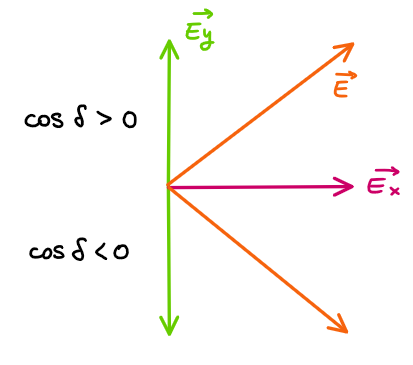
\includegraphics[width=0.34\textwidth]{fotos/criterio signos t0.png}}
    \hspace{2cm}
      \subfloat[Propagación en $t = \sfrac{T}{4}$]{
        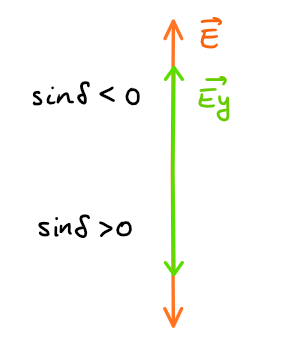
\includegraphics[width=0.25\textwidth]{fotos/criterio signos tT4.png}}
    \end{figure}\\
    
    \noindent A partir de las ecuaciones y de estos esquemas hemos tomado el siguiente como criterio de signos:\\
    
    \begin{tcolorbox}[colback=gris,colframe=azuloscuro,title=Criterio de signos respecto a las ecuaciones de onda vistas en teoría]
    \begin{itemize}
        \item \textbf{Polarización dextrógira}: $-\pi < \delta < 0$
        \item \textbf{Polarización levógira}: $0 < \delta < \pi$
    \end{itemize}
    \end{tcolorbox}\label{box:criterio teoria}
    
    \noindent Cuando nos disponemos a trabajar con el programa, vemos que las ecuaciones que describen las ondas de campo electromagnético son las siguientes:
    \begin{equation}
    \left\{ \begin{array}{lr} \Vec{E_p} = \hat{i}A_{p} cos(wt-kz) \\
    \Vec{E_s} = \hat{j}A_{s} cos(wt-kz+\delta)  \end{array} \right.
    \end{equation}\label{eq:campo em programa}
    
    \noindent Si comparamos este par de ecuaciones con las que se muestran en \ref{eq:onda em teoria}, vemos que la diferencia más importante es que en lo que respecta a la variable contenida en el coseno, ahora la parte que queda positiva es la temporal - $wt$ - mientras que antes la parte positiva era la espacial - $kz$.
    ¿Cómo afecta esto al criterio de signos para la polarización dextógira y levógira? \\

    \noindent Vamos a llamar $\delta '$ al desfase tomando la ecuación de onda tal y como lo hace el programa. Nuestro objetivo es buscar la relación que tiene con $\delta$, que corresponde al desfase que hemos visto en la teoría y basado en el cual ya tenemos un criterio de signos sólido. Para ello, hemos de tener en cuenta una propiedad muy importante del coseno: es una función par, es decir, $cos(x) = cos(-x)$. A fin de comparar ambas expresiones para las ondas electromagnéticas, vamos a reescribir \ref{eq:campo em programa} de forma que dentro del coseno la parte positiva sea la espacial (de forma análoga a \ref{eq:onda em teoria}).
    \begin{equation*}
    \left\{ \begin{array}{lr} \Vec{E_p} = \hat{i}A_{p} cos(wt-kz) \\
    \Vec{E_s} = \hat{j}A_{s} cos(wt-kz+\delta ')  \end{array} \right. \stackrel{cos(-x) = cos(x)}{\Longrightarrow} 
    \left\{ \begin{array}{lr} \Vec{E_p} = \hat{i}A_{p} cos(kz-wt) \\
    \Vec{E_s} = \hat{j}A_{s} cos(kz-wt-\delta ')  \end{array} \right.
    \end{equation*}
    \noindent Igualando una a una las ecuaciones encontramos la siguiente relación:
    \begin{equation}
        cos(kz-wt-\delta ') = cos(wt-kz+\delta) \Longrightarrow kz-wt-\delta ' = wt-kz+\delta \Longrightarrow \delta ' = - \delta
    \end{equation}
    \noindent Ahora que hemos relacionado el desfase obtenido partiendo de ambos planteamientos, y sabiendo que nuestro criterio hasta el momento ha sido \ref{box:criterio teoria}, podemos establecer este nuevo criterio de signos para el programa empleado:\\
    
    \begin{tcolorbox}[colback=gris,colframe=azuloscuro,title=Criterio de signos respecto a las ecuaciones de onda que usa el programa]
    \begin{itemize}
        \item \textbf{Polarización dextrógira}: $0 < \delta < \pi$
        \item \textbf{Polarización levógira}: $-\pi < \delta < 0$
    \end{itemize}
    \end{tcolorbox}\label{box:criterio programa}
    
    \subsection{Justificación de los signos en la definición de los parámetros de Stokes}
    \noindent Recordamos, por lo visto en la parte teórica de la asignatura, que los parámetros de Stokes son un conjunto de valores que nos describen y ayudan a comprender el estado de polarización de las ondas electromagnéticas. En forma matricial y normalizados (puesto que el primero de sus coeficientes toma valor $S_0 = 1$) se pueden escribir de la siguiente forma:
    \begin{equation}
    {\displaystyle {\vec {S}}\ ={\begin{pmatrix}S_{0}\\S_{1}\\S_{2}\\S_{3}\end{pmatrix}}={\frac{1}{E_{ox}^2+E_{oy}^2}\begin{pmatrix}E_{ox}^2+E_{oy}^2\\E_{ox}^2-E_{oy}^2\\2E_{ox}E_{oy}cos(\delta)\\-2E_{ox}E_{oy}sin(\delta)\end{pmatrix}}}
    \end{equation} \label{eq:stokes teoria}
    
    \noindent En relación con estos parámetros hemos establecido un nuevo criterio de signos para determinar el tipo de polarización con el que trabajamos.
    
    \begin{tcolorbox}[colback=gris,colframe=azuloscuro,title=Criterio de signos respecto a los parámetros de Stokes]
    \begin{itemize}
        \item \textbf{Polarización dextrógira}: $S_3 > 0$
        \item \textbf{Polarización levógira}: $S_3 < 0$
    \end{itemize}
    \end{tcolorbox}\label{box:criterio Stokes}
    
    \noindent En el programa los parámetros, además de tener otra nomenclatura relacionada con el significado físico de cada uno de ellos, se definen de forma distinta:
    \begin{equation}
    {\displaystyle {\vec {S}}\ ={\begin{pmatrix}I\\M\\C\\S\end{pmatrix}}={\frac{1}{A_{p}^2+A_{s}^2}\begin{pmatrix}A_{p}^2+A_{s}^2\\A_{p}^2-A_{s}^2\\2A_{p}A_{s}cos(\delta ')\\2A_{p}A_{s}sin(\delta ')\end{pmatrix}}}
    \end{equation} \label{eq:stokes programa}
    
    \noindent Puesto que el parámetro que rige el criterio de signos ahora está en positivo, intuitivamente podríamos pensar que dicho criterio queda alterado. Sin embargo, al analizar bien las ecuaciones vemos que no cambia en absoluto: su valor positivo corresponde a una polarización dextrógira, y el negativo, a la levógira. ¿Cómo es esto posible? \\

    \noindent Llegados a este punto vamos a trabar únicamente con el cuarto parámetro de Stokes, que en la teoría hemos llamado $S_3$ y en el programa, $S$. Para justificar la definición de $S$ con un signo negativo, hemos de tener en cuenta una de las propiedades clave de la función seno: es una función impar, lo cual implica que $sin(-x) = -sin(x)$. Partiendo de las expresiones de $S$ y $S_3$ y recordando que para el programa el desfase es $\delta ' = - \delta$:
    \begin{equation}
    \begin{split}
        A_{p}A_{s}sin(\delta ') = -2E_{ox}E_{oy}sin(\delta) \Longrightarrow sin(\delta ') = -sin(\delta) \Longrightarrow \\ \stackrel{\delta ' = - \delta}{\Longrightarrow} sin(-\delta) = -sin(\delta) \stackrel{sin(-x) = -sin(x)}{\Longrightarrow} -sin(\delta) = -sin(\delta)
    \end{split}
    \end{equation}
    \noindent Hemos llegado a que ambos coeficientes son iguales, y con ello hemos justificado la definición con un signo $+$ del parámetro $S$ así como la no incongruencia en el criterio de signos \ref{box:criterio Stokes}.
    \subsection{Deducción del coeficiente $r_p$ e interpretación de las ecuaciones de Fresnel}
    \noindent Las ecuaciones de Fresnel son un conjunto de expresiones que nos ayudan a comprender la relación entre la amplitud de una onda que incide en un material respecto a la amplitud de la onda que se refleja o se transmite en la interfase. Ahora $\delta$ será la diferencia de fase entre la onda reflejada y la transmitida.\\

    \noindent Estos coeficientes se dividen según si se refieren a la parte de la onda que es paralela o perpendicular al plano de incidencia. De la misma forma, tenemos un par de coeficientes para la onda que se refleja - los coeficientes de reflexión $r_\perp$ y $r_\parallel$ - y otro par para la onda transmitida - los coeficientes de transmisión $t_\perp$ y $t_\parallel$. En este apartado vamos a centrarnos únicamente en el coeficiente de la onda reflejada paralelamente al plano de incidencia, $r_\parallel \equiv r_p$.\\ 

    \begin{wrapfigure}[12]{r}{0.49\textwidth}
        \vspace{-0.5cm}
        \centering
        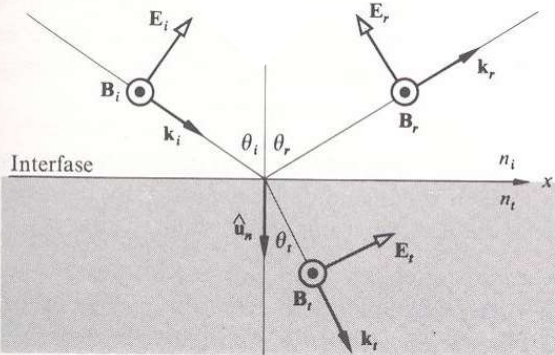
\includegraphics[width=0.45\textwidth]{fotos/criterio_teoría.png}
    \end{wrapfigure}
    
    \noindent En este primer esquema - tomado, al igual que el siguiente, del material introductorio de la práctica - se refleja cómo hemos tomado nuestro criterio en la parte teórica de la asignatura. Vemos que el campo eléctrico reflejado y transmitido se toman en la misma orientación. \\
    
    \noindent Si desarrollamos teniendo en cuenta que estamos en un dieléctrico queda lo siguiente:
    \begin{equation}
        \begin{split} 
        r_\parallel={\frac {n_{t}\cos \theta _{i}-n_{i}\cos \theta _{t}}{n_{i}\cos \theta _{t}+n_{t}\cos \theta _{i}}}
        \Longrightarrow
        \left\{ \begin{array}{lr} r_\parallel > 0 \Longrightarrow \delta = 0\\ r_\parallel < 0 \Longrightarrow \delta = \pi \end{array} \right.     
        \end{split}
    \end{equation}\\
    
    \begin{wrapfigure}[10]{l}{0.49\textwidth}
        \vspace{-0.5cm}
        \centering
        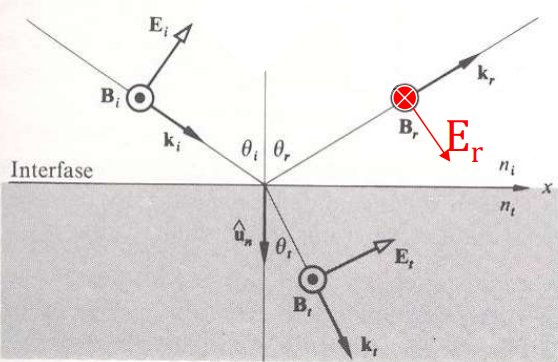
\includegraphics[width=0.45\textwidth]{fotos/criterio_programa.png}
    \end{wrapfigure}
    \noindent Ahora comparemos este caso con el planteamiento que propone el programa \textit{JavaOptics}.\\
    
    \noindent En esta imagen, análoga a la anterior, se ha marcado en rojo la diferencia principal entre ambos planteamientos. En este caso la parte de la onda correspondiente al campo eléctrico reflejado apunta hacia abajo, por lo que hemos de contar con una diferencia de fase $\delta_{inicial} = \pi$.\\
    
    \noindent ¿Cómo deducimos ahora $r_p$? En primer lugar, hemos de considerar el ángulo de incidencia y de reflexión iguales: $\theta_i = \theta_t$. Ahora aplicamos la condición de interfase (únicamente para el campo eléctrico):
    \begin{equation*}
        E_{ix} + E_{rx} = E_{lx} \Longrightarrow E_icos(\theta_i) + E_rcos(\theta_r) = (E_i + E_r)cos(\theta_i) = E_tcos(\theta_t) 
    \end{equation*}
    
    \noindent A partir de aquí despejamos el campo eléctrico transmitido:
    \begin{equation}
        E_t = (E_i+E_r)\frac{cos(\theta_i)}{cos(\theta_t)}
    \end{equation} \label{eq:paso1}

    \noindent Dejamos esto por aquí y nos preguntamos cuál es la expresión que define cada componente del campo eléctrico. Vamos a escribir la expresión general y luego tendremos en cuenta que se han de cumplir para todo punto del espacio y para todo instante del tiempo.
    \begin{equation*}
    \left\{ \begin{array}{lr} E_i = E_{oi}cos(w_it-k_{ix}x) \\ E_r = E_{or}cos(w_rt-k_{rx}x-k_{rz}z)\\
    E_t = E_{ot}cos(w_tt-k_{tx}x-k_{tz}z)
    \end{array} \right. \Longrightarrow \left\{ \begin{array}{lr} E_i = E_{oi}\\ E_r = E_{or}\\
    E_t = E_{ot} \end{array} \right.
    \end{equation*}
    \noindent Aplicando esto en la condición obtenida en \ref{eq:paso1}:
    \begin{equation}
        E_{ot} = (E_{oi}+E_{or})\frac{cos(\theta_i)}{cos(\theta_t)}
    \end{equation} \label{eq:paso2}
    \noindent Para seguir desarollando nuestras expresiones y llegar hasta $r_p$, hemos de remitirnos a la condición de frontera para el campo magnético y tener en cuenta que $B = \frac{n}{c}E$.
    \begin{equation}
        \frac{B_i}{\mu_i} - \frac{B_r}{\mu_r} = \frac{B_t}{\mu_t} \Longrightarrow \frac{n_i}{c\mu_i}E_{oi} - \frac{n_r}{c\mu_r}E_{or} = \frac{n_t}{c\mu_t}E_{ot} = (E_{oi}+E_{or})\frac{cos(\theta_i)}{cos(\theta_t)}\frac{n_t}{c\mu_t}
    \end{equation}
    \noindent Aplicando la condición para las amplitudes del campo y reorganizando los términos nos quedará lo siguiente:
    \begin{equation}
        -E_{or}\left(\frac{n_i}{\mu_i}cos(\theta_t)+\frac{n_t}{\mu_t}cos(\theta_i)\right) = E_{oi}\left(\frac{n_t}{\mu_t}cos(\theta_i)+\frac{n_i}{\mu_i}cos(\theta_t)\right)
    \end{equation}
    \noindent Finalmente tendremos en cuenta que trabajamos en un dieléctrico, y por tanto $\mu_0 = \mu_i = \mu_t$ y que por definición $r_p = \frac{E_{or}}{E_{oi}}$:
    \begin{equation}
        r_p=-{\frac {n_{t}\cos \theta _{i}-n_{i}\cos \theta _{t}}{n_{i}\cos \theta _{t}+n_{t}\cos \theta _{i}}} = -r_\parallel
    \end{equation}
    \noindent ¿Cómo queda el criterio de signos en este caso? Solo hemos de tener en cuenta el cambio de signos respecto a la ecuación teórica.
    \begin{equation}
        \begin{split}
            \left\{ \begin{array}{lr} r_p > 0 \Longrightarrow \delta = \pi\\ r_p < 0 \Longrightarrow \delta = 2\pi = 0 \end{array} \right. 
        \end{split}
    \end{equation}
    \newpage 
    \section{Polarización}
    \noindent En esta segunda sección vamos a estudiar distintos estados de polarización, en concreto los parámetros de amplitud y desfase elegidos para obtener cada caso. También explicaremos la información que nos aportarán los parámetros de Stokes y deduciremos gráficamente el valor del desfase.
    \subsection{Luz linealmente polarizada a $\alpha = 60^o$}
    \begin{wrapfigure}[12]{l}{0.45\textwidth}
        \vspace{-0.5cm}
        \centering
        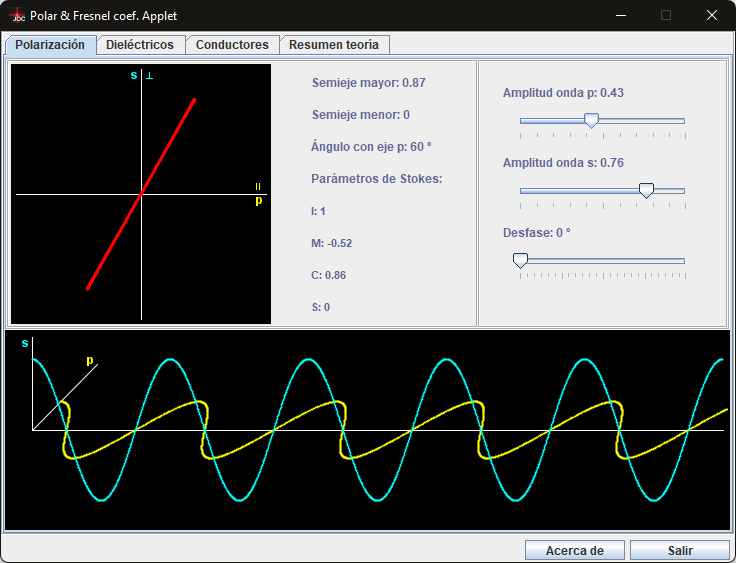
\includegraphics[width=0.45\textwidth]{fotos/luz lin pol 60.png}
    \end{wrapfigure}
    
    \noindent Se trata de una luz lineal con pendiente positiva, por lo que el desfase que hemos de tomar es $\delta = 0^o$. En lo que respecta a la amplitud, hemos tomado $A_s > A_p$ porque la pendiente es mayor a $45^o$. \\
    
    \noindent Es precisamente esta desigualdad la que causa $M < 0$ (para comprobarlo solo hace falta ver cómo lo hemos definido en \ref{eq:stokes programa}). En lo que respecta al resto de parámetros de Stokes, es notable que $S = 0$ porque la luz está polarizada de forma lineal y por ello no puede ser levógira ni dextrógira.\\

    \noindent Al fijarnos en la gráfica - donde $\Vec{E_\parallel}$ viene representado en amarillo y $\Vec{E_\perp}$, en azul - vemos que sus máximos coinciden en el mismo punto. Esto coincide con el valor nulo del desfase tal y como ya lo habíamos comentado.
    
    \subsection{Luz linealmente polarizada a $\alpha = -30^o$}
    \begin{wrapfigure}[12]{r}{0.45\textwidth}
        \vspace{-0.25cm}
        \centering
        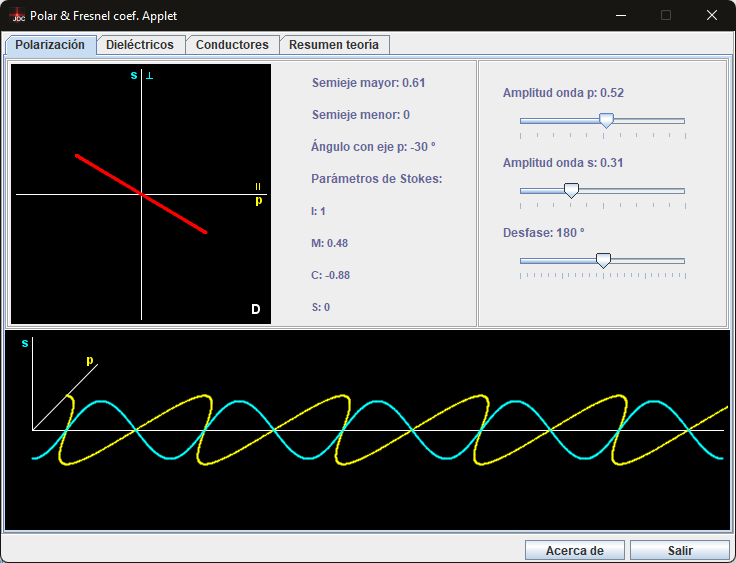
\includegraphics[width=0.45\textwidth]{fotos/luz lin pol -30.png}
    \end{wrapfigure}
    \noindent Esta luz sigue estando linealmente polarizada, pero ahora $\alpha = -30^o$. Es precisamente por este valor del ángulo negativo pero mayor a $-45^o$ por lo que ahora $Ap > As$. Por la propia definición de $M$, ahora tomará un valor positivo.\\

    \noindent En cuanto al parámetro S, sigue tomando valores nulos por la misma razón que antes. Sin embargo, otra de las magnitudes que cambia es el desfase, puesto que ahora $\delta = 180^o$. Esto se corrobora en el dibujo: cuando la onda perpendicular llega a su máximo, la paralela se encuentra en su mínimo.
    
    \newpage
    \subsection{Luz circular dextrógira}
    \begin{wrapfigure}[12]{r}{0.45\textwidth}
        \vspace{-0.5cm}
        \centering
        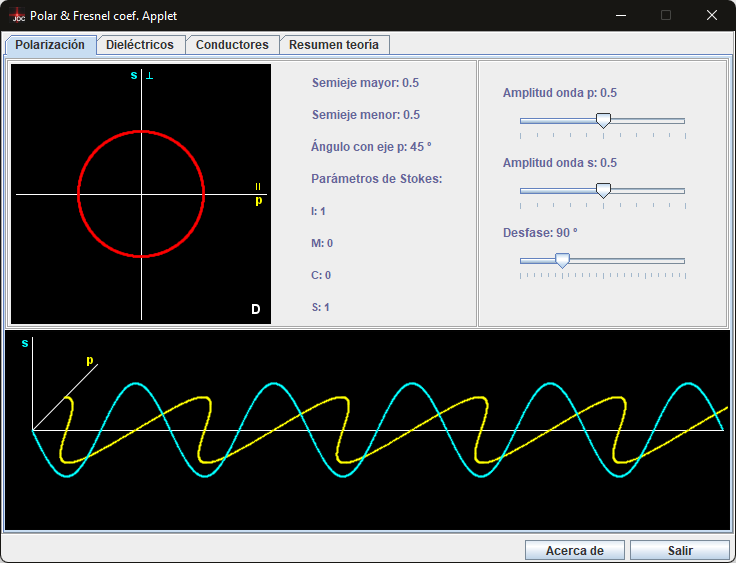
\includegraphics[width=0.45\textwidth]{fotos/luz circular dextrógira.png}
    \end{wrapfigure}
    \noindent Ahora ya no tenemos una luz linealmente polarizada, sino que es circular: es por ello que hemos tomado las amplitudes iguales, $A_s = A_p$. Si no fueran iguales, la luz sería elíptica. El desfase ahora es $\delta = \frac{\pi}{4}$ porque es luz dextrógira - esto se comprueba en la gráfica puesto que cuando una de las dos componentes del campo eléctrico alcanza un extremo relativo, la otra se anula. \\

    \noindent Al remitirnos a los parámetros de Stokes, vemos que por su definición tanto $M$ como $C$ son nulos. Como la luz está polarizada de forma dextrógira, vemos que $S = 1 > 0$, lo cual coincide con lo que hemos desarrollado en la teoría.

    \subsection{Luz elípticamente polarizada, dextrógira con semieje mayor horizontal}
    \begin{wrapfigure}[6]{l}{0.45\textwidth}
        \vspace{-0.5cm}
        \centering
        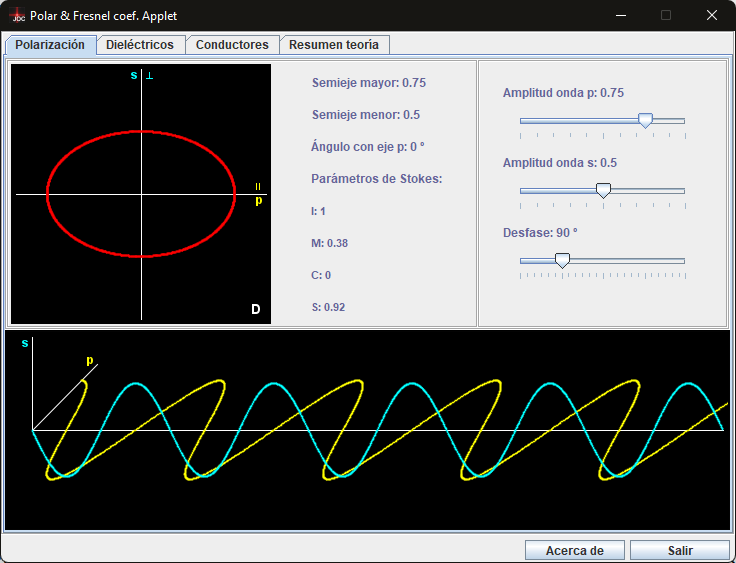
\includegraphics[width=0.45\textwidth]{fotos/eliptica dext smh.png}
    \end{wrapfigure}
    \noindent La luz en este caso está polarizada elípticamente con semieje mayor horizontal, por lo que la amplitud de onda paralela ha de ser mayor a la amplitud de onda perpendicular ($A_p > A_s$). Por ser dextrógira, la justificación tanto de los parámetros de Stokes como del desfase es análoga a la del apartado anterior.\\
    \vspace{2.3cm}
    \subsection{Luz elípticamente polarizada, levógira con semieje mayor vertical}
    \begin{wrapfigure}[12]{r}{0.45\textwidth}
        \vspace{-0.5cm}
        \centering
        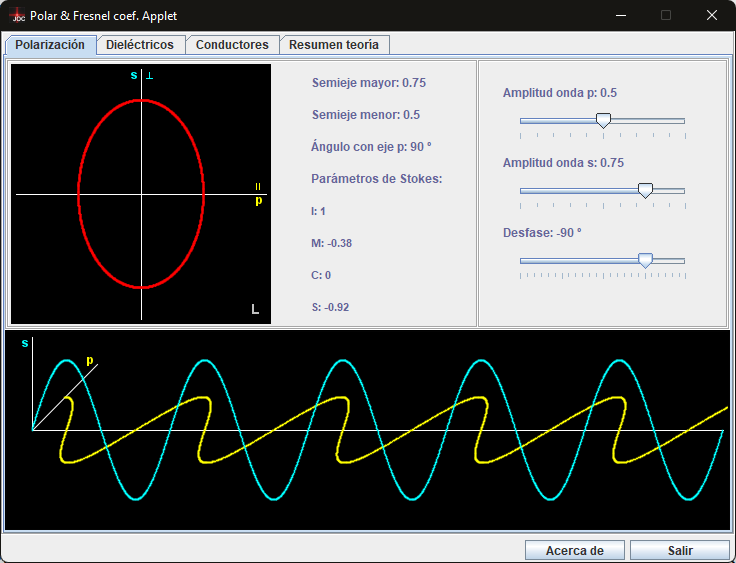
\includegraphics[width=0.45\textwidth]{fotos/eliptica lev smh.png}
    \end{wrapfigure}
    \noindent Este caso es muy similar al anterior, pero como ahora el semieje mayor es el vertical, la amplitud mayor será la perpendicular, $A_s > A_p$. Ahora la onda está polarizada de forma levógira, por lo que $\delta = -\frac{\pi}{4}$: a nivel gráfico, vemos lo mismo que en los dos casos anteriores. \\

    \noindent En lo respectivo al los parámetros de Stokes, vemos que por definición $M < 0$, $C = 0$ y por ser luz levógira se comprueba, tal y como hemos deducido en la teoría, que $S < 0$.
    \newpage
    \subsection{Luz elípticamente polarizada dextrógira con inclinación $\psi = 30^o$}
    \begin{wrapfigure}[8]{l}{0.45\textwidth}
        \vspace{-0.6cm}
        \centering
        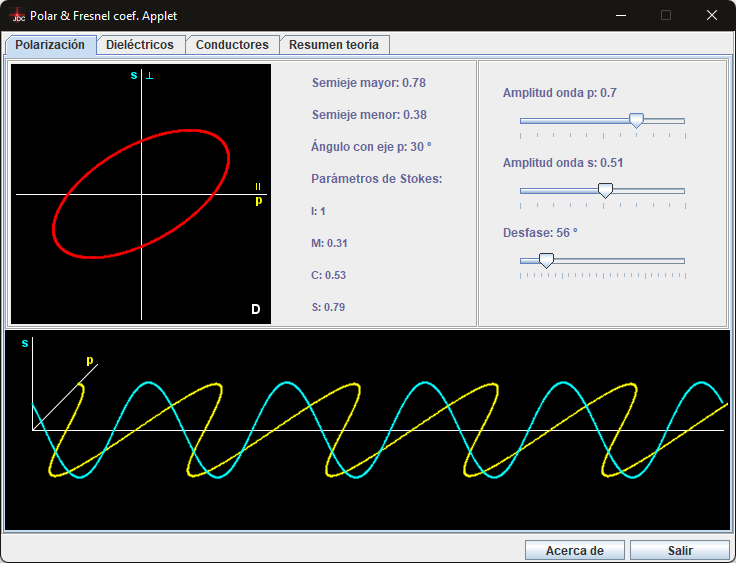
\includegraphics[width=0.45\textwidth]{fotos/eliptica dext 30.png}
    \end{wrapfigure}
    \noindent ¿Cómo conseguimos una elipse inclinada? Vamos a relacionarlo con el parámetro asociado a la inclinación mediante la siguiente expresión:
    \begin{equation}
    \begin{split}
        tan(2\psi) = \frac{2A_pA_scos(\delta)}{A_p^2-A_s^2} \\\Longrightarrow \delta = arccos\left(\frac{(A_p^2-A_s^2)tan(60^o)}{2A_pA_s}\right)
    \end{split}
    \end{equation}
    \noindent Si sustituimos en esta expresión los valores de las amplitudes nos queda $\delta = 53.56^o$.\\

    \noindent En lo que respecta a los parámetros de Stokes, $M > 0$ por ser la amplitud de la onda paralela mayor a la perpendicular, y $S > 0$ por ser luz dextrógira.
    
    
    \newpage
    \section{Dieléctricos}
    
        \begin{table}[ht]
            \centering
            \resizebox{\textwidth}{!}{%
            \begin{tabular}{|cccccc|}
                \hline
                \rowcolor[HTML]{010066} 
                \multicolumn{6}{|c|}{\cellcolor[HTML]{010066}{\color[HTML]{FFFFFF} \textbf{REFLEXIÓN EXTERNA}}} \\ \hline
                \rowcolor[HTML]{CBCEFB} 
                \multicolumn{1}{|c|}{\cellcolor[HTML]{CBCEFB}$\theta_i$} &
                  \multicolumn{1}{c|}{\cellcolor[HTML]{CBCEFB}$\text{Ap}_r=\left|rp\right|\text{Ap}_i$} &
                  \multicolumn{1}{c|}{\cellcolor[HTML]{CBCEFB}{\color[HTML]{000000} $\text{As}_r=\left|rs\right|\text{As}_i$}} &
                  \multicolumn{1}{c|}{\cellcolor[HTML]{CBCEFB}$\delta r=\delta_sr-\delta_pr$} &
                  \multicolumn{1}{c|}{\cellcolor[HTML]{CBCEFB}$\delta r -\text{tot}=\delta_i+\delta_r$} &
                  \textbf{Tipo de luz reflejada} \\ \hline
                \multicolumn{1}{|c|}{\cellcolor[HTML]{FFFFFF}$45^\circ$} &
                  \multicolumn{1}{c|}{} &
                  \multicolumn{1}{c|}{} &
                  \multicolumn{1}{c|}{} &
                  \multicolumn{1}{c|}{} &
                   \\
                \rowcolor[HTML]{EFEFEF} 
                \multicolumn{1}{|c|}{\cellcolor[HTML]{EFEFEF}$59.5^\circ$} &
                  \multicolumn{1}{c|}{\cellcolor[HTML]{EFEFEF}} &
                  \multicolumn{1}{c|}{\cellcolor[HTML]{EFEFEF}} &
                  \multicolumn{1}{c|}{\cellcolor[HTML]{EFEFEF}} &
                  \multicolumn{1}{c|}{\cellcolor[HTML]{EFEFEF}} &
                   \\
                \multicolumn{1}{|c|}{\cellcolor[HTML]{FFFFFF}$80^\circ$} &
                  \multicolumn{1}{c|}{} &
                  \multicolumn{1}{c|}{} &
                  \multicolumn{1}{c|}{} &
                  \multicolumn{1}{c|}{} &
                   \\ \hline
                \rowcolor[HTML]{CBCEFB} 
                \multicolumn{1}{|c|}{\cellcolor[HTML]{CBCEFB}$\theta_i$} &
                  \multicolumn{1}{c|}{\cellcolor[HTML]{CBCEFB}$\text{Ap}_t=\left|tp\right|\text{Ap}_i$} &
                  \multicolumn{1}{c|}{\cellcolor[HTML]{CBCEFB}$\text{As}_t=\left|ts\right|\text{As}_i$} &
                  \multicolumn{1}{c|}{\cellcolor[HTML]{CBCEFB}$\delta t=\delta_st-\delta_pt$} &
                  \multicolumn{1}{c|}{\cellcolor[HTML]{CBCEFB}$\delta t -\text{tot}=\delta_i+\delta_t$} &
                  \textbf{Tipo de luz transmitida} \\ \hline
                \multicolumn{1}{|c|}{\cellcolor[HTML]{FFFFFF}$45^\circ$} &
                  \multicolumn{1}{c|}{} &
                  \multicolumn{1}{c|}{} &
                  \multicolumn{1}{c|}{} &
                  \multicolumn{1}{c|}{} &
                   \\
                \rowcolor[HTML]{EFEFEF} 
                \multicolumn{1}{|c|}{\cellcolor[HTML]{EFEFEF}$59.5^\circ$} &
                  \multicolumn{1}{c|}{\cellcolor[HTML]{EFEFEF}} &
                  \multicolumn{1}{c|}{\cellcolor[HTML]{EFEFEF}} &
                  \multicolumn{1}{c|}{\cellcolor[HTML]{EFEFEF}} &
                  \multicolumn{1}{c|}{\cellcolor[HTML]{EFEFEF}} &
                   \\
                \multicolumn{1}{|c|}{\cellcolor[HTML]{FFFFFF}$80^\circ$} &
                  \multicolumn{1}{c|}{} &
                  \multicolumn{1}{c|}{} &
                  \multicolumn{1}{c|}{} &
                  \multicolumn{1}{c|}{} &
                   \\ \hline
            \end{tabular}%
            }
            \caption{Reflexión externa}
            \label{tab:reflexion_externa}
        \end{table}
        

\end{document} 